\documentclass[a4paper]{article}

\usepackage{listings}
\usepackage[utf8]{inputenc}
\usepackage[T1]{fontenc}
\usepackage[spanish]{babel}
\usepackage[left=2cm, right=2cm, top=2cm, bottom=2cm]{geometry}
\usepackage{setspace}
\usepackage{graphicx}
\usepackage{xcolor}
\usepackage{geometry}
\usepackage{multirow}
\usepackage[hidelinks]{hyperref}
\usepackage{setspace} % Para el espaciado entre lineas
\setstretch{1.2} % Aquí definimos el espaciado en unidades
\usepackage{parskip} %  Para arreglar la forma en la que se manejan los parrafos
\usepackage{fancyhdr}
\usepackage{tikz,lipsum,lmodern}
\usepackage[most]{tcolorbox}
\usetikzlibrary{shapes.geometric, arrows}
\usepackage{appendix}

% Sets de dimensiones
\setlength{\parindent}{0pt}
\setlength{\parskip}{0.8em plus 0.5em minus 0.2em}
\setlength{\parfillskip}{\parindent plus 1fill}

% Declaración de variables personalizadas
\newcommand{\logoPortada}{Images/PixelartPisa.png}
\newcommand{\cifplogo}{Images/cifplogo.png}

% Definición de colores
\definecolor{bluePortada}{HTML}{146c8a}

%Adicionales
\setlength{\headheight}{40.2pt}
\pagestyle{fancy}
\fancyhf{}
\lhead{\includegraphics[width=1cm]{\logoPortada}}\rhead{
\includegraphics[width=2cm]{Images/cifplogo.png}}
\renewcommand{\headrulewidth}{3pt}
\renewcommand{\headrule}{\hbox to\headwidth{\color{bluePortada}\leaders\hrule height \headrulewidth\hfill}}

\tikzstyle{startstop}=[rectangle,rounded corners, minimum width=3cm,minimum height= 1cm, text centered,draw=black, fill=red]
\tikzstyle{io}=[trapezium,trapezium left angle=70,trapezium right angle=110,minimum width=3cm,minimum height= 1cm, text centered,draw=black, fill=blue]
\tikzstyle{process}=[rectangle,minimum width=3cm,minimum height= 1cm, text centered,text width= 3cm,draw=black, fill=orange]
\tikzstyle{decision}=[diamond,minimum width=3cm,minimum height= 1cm, text centered,draw=black, fill=green]
\tikzstyle{arrow}=[thick]



\begin{document} % Inicio del documento
\begin{titlepage}
    \centering % para centrar
    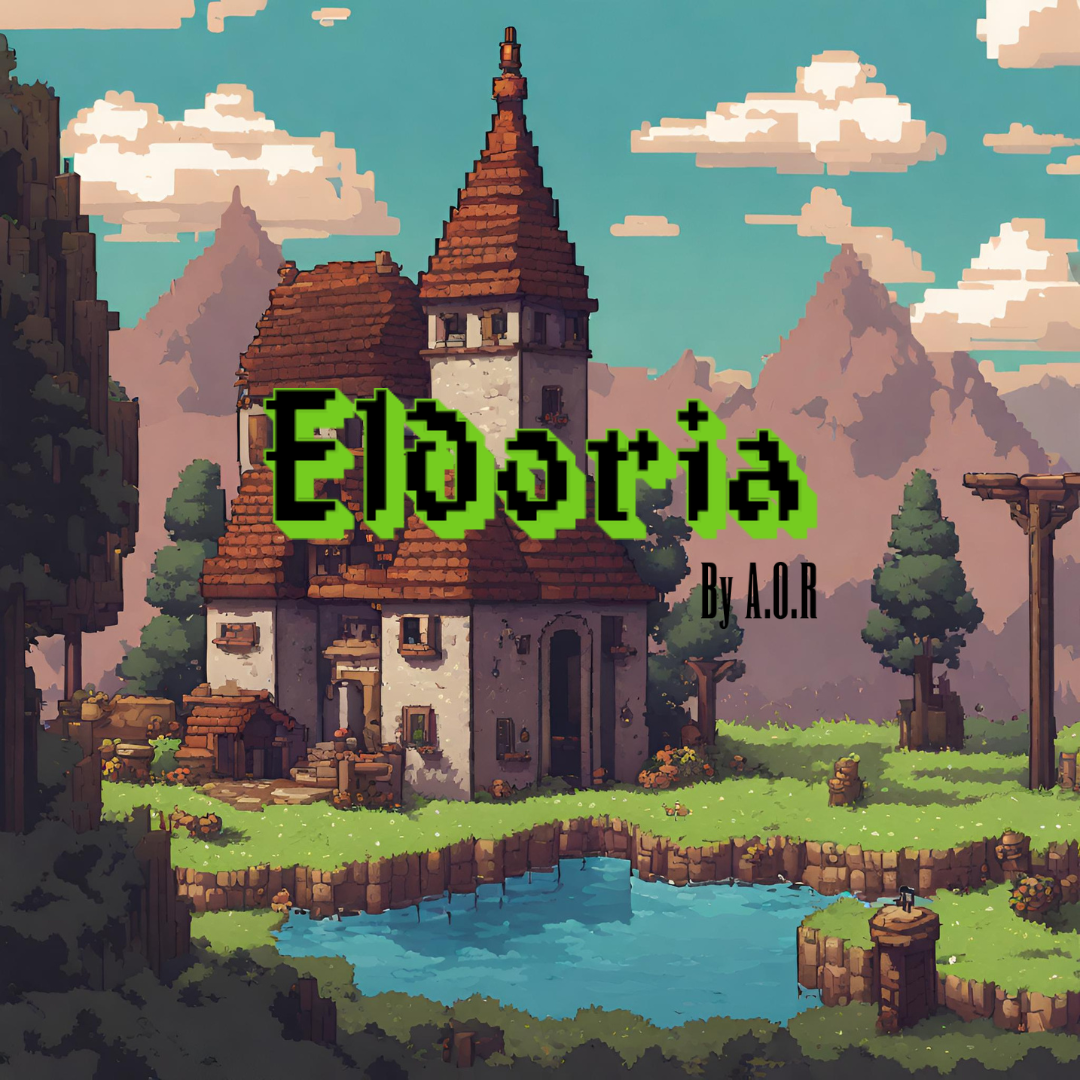
\includegraphics[width=0.5\textwidth]{Images/Eldoria.png}\par
    \vspace{0.4cm}
    {\scshape\LARGE\textbf{TFG DAM - CIFP LaLaboral}\par} % Contenido de la portada
    \vspace{0.4cm}
    {\LARGE\textcolor{bluePortada}{Eldoria - Alejandro Orviz Recalde}\par}
\end{titlepage}
% Comienzo del TOC
\clearpage
\tableofcontents
\clearpage
% ---------------------------------------------------------------------
\section{Agradecimientos}
Este proyecto no seria posible sin la ayuda de varias personas involucradas en este desarrollo. Carles por ayudarme con sus reviews de código,
Laura por darme parte de sus conocimientos en el desarrollo de videojuegos para poder desarrollar bien, Marta la tutora por resolverme dudas y otorgarme
documentación, y por ultimo Miguel por haberme inspirado a realizar este videojuego, el cual está dedicado hacia él.

Las funciones de estas personas me han ayudado en mayor o menor medida a terminar este TFG, el cual no podría haber acabado sin ayuda, es por ello que reservo
esta parte del docuemnto para agradecer a estar personas su colaboración conmigo, sobre todo a Carles y Laura, los cuales me han apoyado durante todo el desarollo.
\clearpage
% ---------------------------------------------------------------------
\section{Introducción}
El presente proyecto trata sobre un Juego llamado \textbf{Eldoria}, se encuentra desarrollado en \textit{Java} y es una aventura en 2 dimensiones con graficos \textit{pixel art}
el cual tendra una forma de jugar similar a videojuegos antiguos tales como:
\begin{itemize}
    \item The legend of Zelda
    \item The legend of Zelda Minish cap
    \item Final Fantasy I, II, III
    \item Super Mario RPG
\end{itemize}
Algunos datos del proyecto adicionales son:

\begin{center}
    \begin{tabular}{| c | c |}
        \hline
        Titulo de la aplicacion   & Eldoria         \\ \hline
        Autor                     & Alejandro Orviz \\ \hline
        Profesor                  & Alberto         \\ \hline
        Tutora                    & Marta           \\ \hline
        Code reviews              & Carles          \\ \hline
        Desarrollo de videojuegos & Laura           \\ \hline
    \end{tabular}
\end{center}

El videojuego se inspira fuertemente en los primeros juegos creados para la Super Nintendo, por lo que se veran bastantes similitudes tanto en estructura de niveles
como en linealidad e historia del mismo. Ademas todas las images que se han usado son libres de derechos de autor o en su defecto creadas con inteligencia artificial para evitar problemas de copyright.

\clearpage
% ----------------------------------------------------
\subsection{Motivación}
A dia de hoy son muchas las personas que juegan a videojuegos, pero no muchos recuerdan las bases u origenes de los mismos, en este caso, en mi juego llamado
\textbf{Eldoria} tenemos una aventura en 2 dimensiones en estetica \textit{pixel} que nos lleva a un mundo de fantasia el cual nos puede provocar la nostalgia de revivir
videojuegos como \textit{The legend of Zelda 1}. Ademas este videojuego aprovecha conceptos de programacion sobre lectura, apertura y creacion de archivos asi como
conexiones con bases de datos. La duracion del mismo aun esta por determinar y depende mas bien de la persona y del tipo de jugador. Con este proyecto se busca
es proveer al usuario de un tiempo de ocio en el que pueda disfrutar pasando el tiempo frente a retos y acertijos propuestos por el videojuego.

\subsection{Inspiraciones}
Este juego además tiene varias inspiraciones en el mundo moderno y \textit{retro}, pasaremos a explicar en profundidad sus inspiraciones, las cuales incluyen tambien documentos realizados por otra gente como veremos a contiuación:\\
\begin{enumerate}
    \item \textbf{The legend of Zelda}
          \begin{itemize}
              \item \textit{The legend of Zelda} es un videojuego japonés de los años 80, el cual fue desarrollado por Nintendo. Se trata de un videojuego de aventuras, puzzles y acción, fue un referente en su época y a día de hoy se considera la base de los juegos de aventuras.
              \item El objetivo dentro del juego es simple, nuestro protagonista \textit{Link}, debe rescatar a la princesa \textit{Zelda} de las garras del \textit{Rey Demonio}, para ello tendrá que recorrer \textit{Hyrule} en busca de objetos, armas, conocimiento, etc \dots
              \item Hablando de temas tecnicos, el juego se considera un \textit{RPG (Role playing game)}, es decir, un juego de rol, de perspectiva aérea que cuenta con varios puzzles para superar algún nivel. En tema de gráficos, encontramos una estética \textit{pixel art} la cual, no requiere un desarrollo super extenso.
              \item Aunque a día de hoy existen varios videojuegos de \textit{The legend of Zelda}, nosotros nos fijaremos en el primero ya que es el que dejó las bases para el resto de los juegos de la saga, es por eso que el videojuego, en estética y jugabilidad, bebe mucho de esta obra.
          \end{itemize}
    \item \textbf{Final fantasy}
          \begin{itemize}
              \item \textit{Final fantasy} es un videojuego de rol japonés desarrollado por \textit{Square.Co(Más tarde conocida como "Square Enix")}, el cual fue un gran pilar en la industria de los videojuegos de rol de la época y actuales, salió en el año 1987, y fue el inicio de una saga de videojuegos que a día de hoy continua su desarrollo(\textit{Actualmente existe el "Final Fantasy XVI"})
              \item La historia de este juego, trata acerca de 4 personajes que van en busca de unos cristales mágicos para vencer el mal que acecha el mundo, esta historia se repetirá en mayor o menor medidad en los próximos juegos de la saga. Su estética es similar al juego previo hablado, \textit{The legend of Zelda}, pues ambos juegos salieron casi en el mismo año y en una época donde el hardware, no era tan potente como ahora.
          \end{itemize}
    \item \textbf{TFG de la Escuela de ingenieria de Segovia}
          \begin{itemize}
              \item Para este proyecto primero, hemos investigado las opciones ya creadas por la gente, en caso de que existieran, en este caso hemos encontrado un TFG (\textit{Estará adjuntado en la parte de Bibliografia}), el cual nos habla acerca del desarrollo de un videojuego móvil con unity, este TFG, nos ha servido de ayuda ya que nos ha provisto de una estructura de desarrollo, enlaces de interés e ideas para el desarrollo.
          \end{itemize}
\end{enumerate}

\subsection{Herramientas usadas}
En esta sección, explicaremos brevemente las herramientas usadas, y el por qué de las mismas, asi como su coste en el caso de que sean de pago.

Para el desarrollo de este TFG, se han usado las siguientes herramientas:
\begin{enumerate}
    \item \textbf{IntelliJ Idea Community y Ultimate}
          \begin{itemize}
              \item \textit{IntelliJ} es nuestro IDE de preferencia, el cual nos provee de varias herramientas utiles y necesarias para el desarrollo del proyecto, se trata de un entorno de desarrollo, lanzado en 2001, el cual cuenta con dos versiones, una gratuita y otra de pago, en este proyecto usaremos principalmente la gratuita, aunque necesitaremos una funcionalidad de la versión de pago.
              \item Este entorno de desarrollo cuenta con una tecnología de sugerencias de código real, bastante avanzada la cual nos provee de código por lo general bastante acertado según lo que estamos desarrollando, ya que mientras programamos, el IDE, analiza lo que estamos escribiendo y lo que hemos programado para darnos mejores sugerencias de autocompletado.
              \item \textbf{El precio de este IDE, actualmente(2024) es de: 160 euros al mes}
          \end{itemize}
    \item \textbf{Docker}
          \begin{itemize}
              \item \textbf{Docker} se trata de un proyecto de código abierto, que nos permite automatizar y facilitar el despliegue de aplicaciones dentro de \textit{contenedores de software}, proporcionando una capa adicional de abstracción y automatización de virtualización de aplicaciones en múltiples sistemas operativos.
              \item \textbf{Docker} ademas está construido sobre las facilidades proporcionadas por el kernel Linux (principalmente cgroups y namespaces), un contenedor Docker, a diferencia de una máquina virtual, no requiere incluir un sistema operativo independiente, por lo que nos permite tener procesos aislados del sistema \textit{"host"} y tener contendores ligeros.
          \end{itemize}
    \item \textbf{Jooq}
          \begin{itemize}
              \item \textbf{Jooq} tambien conocido como Java Object Oriented Querying, es una biblioteca ligera de mapeo de bases de datos que implementa el patrón de registro activo, su proposito es ser tanto relacional como orientada a objetos.
              \item Hemos usado esta biblioteca debido a su similitud con \textit{Linq} el cual es un componente de .NET, que nos permite hacer consultas de una manera muy cómoda.
          \end{itemize}
    \item \textbf{Visual studio Code}
          \begin{itemize}
              \item \textbf{Visual studio Code} es un IDE, que nos provee de una cantidad de configuraciones infinita, y también al tener esta versatilidad es perfecto como IDE, para trabajar en un proyecto que involucre usar varios lenguajes a la vez, aunque en nuestro caso, lo hemos usado para desarrollar el documento \LaTeX, de la memoria del proyecto.
              \item Para desarrollar el documento, hemos tenido que descargarnos \textit{Perl}, \textit{LaTeX Workshop} y por ultimo \textit{MikTex}, esto es necesario si queremos que Visual Studio nos deje desarrollar cualquier docuemnto \LaTeX, además de un plugin para poder visualizar el documento pdf compilado desde Visual Studio.
          \end{itemize}
    \item \textbf{\LaTeX}
          \begin{itemize}
              \item \textbf{\LaTeX} es un sistema de composición de textos orientado a la creación de documentos escritos que presenten una alta calidad tipográfica. Por sus características y posibilidades, se usa de forma especialmente intensa en la generación de artículos y libros científicos que incluyen, entre otros elementos, expresiones matemáticas
              \item \textbf{\LaTeX} está formado por un gran conjunto de macros de \textbf{TeX}, escrito por Leslie Lamport en 1984 con la intención de facilitar el uso del lenguaje de composición tipográfica \LaTeX, creado por Donald Knuth. Se utiliza mucho para la composición de artículos académicos, tesis y libros técnicos, dado que la calidad tipográfica de los documentos realizados en LaTeX se considera adecuada a las necesidades de una editorial científica de primera línea, muchas de las cuales ya lo emplean
              \item Para poder desarrollar el documento de la memoria en \LaTeX, hemos hecho uso de la docuemntación que existe en internet, asi como documentos ya hechos, por ejemplo repositorios de gente que ya ha realizado un documento \LaTeX.
          \end{itemize}
    \item \textbf{MySql}
          \begin{itemize}
              \item \textbf{MySql} es un sistema de gestión de bases de datos relacional desarrollado bajo licencia dual: Licencia pública general/Licencia comercial por \textit{Oracle Corporation} y está considerada como la base de datos de código abierto más popular del mundo, y una de las más populares en general junto a \textit{Oracle} y \textit{Microsoft SQL Server}, todo para entornos de desarrollo web.
              \item \textbf{MySql} fue inicialmente desarrollado por \textit{MySQL AB} (empresa fundada por David Axmark, Allan Larsson y Michael Widenius). \textit{MySQL AB} fue adquirida por \textit{Sun Microsystems} en 2008, y ésta a su vez fue comprada por \textit{Oracle Corporation} en 2010, la cual ya era dueña desde 2005 de Innobase Oy, empresa finlandesa desarrolladora del motor \textit{InnoDB} para \textit{MySQL}.
          \end{itemize}
    \item \textbf{JDK 21}
          \begin{itemize}
              \item \textbf{JDK o \textit{Java Development Kit}} es una seria de herramientas de desarrollo que nos permite crear software en \textit{Java}, ademas de poder ejecutar archivos \textit{"Jar"} desarrollados con esta \textit{JDK}. Hemos decidido usar la última versión para estar libres de problemas de que nos hagan falta paquetes o de vulnerabilidades.
          \end{itemize}
    \item \textbf{Github Repositories}
          \begin{itemize}
              \item Para poder tener un sistema de control de versiones hemos optado por usar los repositorios de \textit{Github}, los cuales de forma gratuita nos dejan tener un sistema de control de versiones que nos permite mantener de forma sincronizada en varios equipos el mismo proyecto, en nuestro caso el repositorio es público, en caso de quererlo privado, tendríamos o bien que pagar o bien disponer de un servidor local con el que poder tener subido el repositorio en él mediante \textit{Git}.
          \end{itemize}
    \item \textbf{Excalidraw}
          \begin{itemize}
              \item \textbf{Excalidraw} es una web que nos ofrece una pizarra virtual en la que poder dibujar, hacer notas o generar diagramas incluso, como los diagramas UML de software, ademas cuenta con bastantes opciones a la hora de exportar lo dibujado, y es una herramienta muy útil para hacer esquemas.
          \end{itemize}
\end{enumerate}
\clearpage
%-----------------------------------------------------
\subsection{Primeras metas}
\begin{enumerate}
    \item \textbf{Realizar un personaje que se mueva en pantalla}
          \begin{itemize}
              \item El principal punto sobre el que podemos avanzar es mostrar el personaje en pantalla y ser capaces de moverlo con las teclas del teclado, que el programa sea capaz de saber si queremos ir a las 4 direcciones posibles y que se mueva con cierta fluidez.
          \end{itemize}

    \item \textbf{60 Frames por segundo}
          \begin{itemize}
              \item Una de las metas tambien principales es limitar el rendimiento del juego ya que queremos que se dibuje lo que hay en pantalla 60 veces por segundo, si no ponemos un limitador, esta cifra sería mucho más alta, lo que nos podria provocar problemas, llegados a un número muy alto de interacciones.
          \end{itemize}

    \item \textbf{Colisiones}
          \begin{itemize}
              \item Dentro de un videojuego queremos que se produzcan colisiones con el personaje o personajes del juego, no queremos que se atraviesen muros, o cosas de ese estilo, por lo que esta es una de las principales metas a superar.
          \end{itemize}

    \item \textbf{Menús de juego}
          \begin{itemize}
              \item También queremos realizar pantallas de estado del personaje, menú principal, dialogos, menú de pausa, etc \dots
          \end{itemize}

    \item \textbf{Sistema de combate}
          \begin{itemize}
              \item Al ser un juego de rol y aventuras, queremos incluir algún enemigo y algun sistema de combate en el que se pueda dar y recibir daño asi como barras de vida para los enemigos, o para el jugador.
          \end{itemize}

    \item \textbf{Pantalla Completa}
          \begin{itemize}
              \item Otra meta seria poder ejecutar el juego en pantalla completa sin bordes, es un pequeño punto de estética.
          \end{itemize}

    \item \textbf{Empaquetar el juego}
          \begin{itemize}
              \item La ultima meta propuesta es empaquetar el juego y poder tener algun ejecutable para poder llevarlo a \textit{"todas partes"}.
          \end{itemize}
\end{enumerate}

\clearpage
% --------------------------------------------
\section{Planificacion y presupuesto}
\subsection{Planificacion}
Este proyecto se ha desarrollado en varias fases como un desarrollo real en un entorno empresarial, empezando en \textit{Octubre de 2023}(los totales de horas son aproximados).
\subsection{Septiembre - 2023}
En esta fase comenzó el descarte de ideas y la lluvia de las misma para saber más o menos que podríamos hacer en cuanto a TFG se refiere
\begin{flushright}
    \bf Total de horas: 10 horas
\end{flushright}

\subsection{Octubre - 2023}
En la primera fase del mismo se ha pensado la idea y hecho una planificacion inicial del mismo, asi como varios apuntes sobre la tecnología a usar, la cual ha recibido cambios en el desarrollo.
\begin{flushright}
    \bf Total de horas: 20 horas
\end{flushright}

\subsection{Noviembre - 2023}
En esta fase empezamos los primeros pasos del desarrollo y encontramos las primeras dificultades del mismo, como por ejemplo:
\begin{itemize}
    \item Assets
    \item Falta de conocimiento
    \item Desconocimiento de la BDD
    \item Diseño de la BDD
\end{itemize}
Teniendo estas dificultades claras continuamos un desarrollo temprano de una pequeña version bastante primitiva del proyecto que nos servirá de base para poder continuar con él. En esta versión declaramos las bases del programa final que tendremos por el final del proyecto.
\begin{flushright}
    \bf Total de horas: 30 horas
\end{flushright}

\clearpage
\subsection{Diciembre - 2023}
En esta fase continuamos un poco mas el desarrollo y adelantamos un poco del mismo de cara a la siguiente fase, ya que en el momento que hemos acabado la fase de primeros pasos el resto que se realice antes del anteproyecto es trabajo adelantado, dentro de esta fase el principal problema que nos hemos encontrado ha sido \textbf{el tamaño del heap de Java}, siendo este el principal limitante a la hora de realizar un diseño de niveles grande como se tenía pensado principalmente. Este problema nos produjo un cambio de planes ya que el mapa que inicialmente se habia pensado en un mapa de 100x100 casillas se tuvo que reducir a 50x50, es decir la mitad, esto nos deja para las pruebas del desarrollo un mapa de 25x25 que más tarde será de 50x50. Este cambio viene de la famosa excepcion \textit{"java.lang.OutOfMemoryError: Java heap space"}.\\
Este problema se produce al dibujar el mapa del videojuego, ya que el heap no es capaz de almacenarlo y entonces nos devuelve esa excepción, para corregirlo, lo que hemos hecho ha sido disminuir el tamaño del mapa a uno más pequeño, si bien es cierto que se puede aumentar la memoria del heap de java mediante comandos, hemos preferido dejarlo como está y disminuir el mapa.\\
Otros datos interesantes de esta fase han sido los progresos en el desarrollo y la nueva replanificación del mismo, ya que al tener el error del heap de java, hemos tenido que reestructurar partes del desarrollo ya planificadas.
\begin{flushright}
    \bf Total de horas: 50 horas
\end{flushright}

\subsection{Enero/Febrero/Marzo - 2024}
Dentro de esta fase tendriamos la parte referente al anteproyecto. El desarrollo del documento del anteproyecto se realizó usando \LaTeX, y \textit{Overleaf (Una pagina dedicada a escribir documentos LaTeX de forma online)}. La plantilla usada en ese documento es una plantilla creada desde cero con los conocimientos de ese momento acerca del lenguaje, y tambien cogiendo cosas de documentación, foros y proyectos ya hechos de otra gente, es el caso de foros como \textit{StackExchange} en su parte referente al lenguaje, repositorios de github con determinadas funciones que he necesitado poner en el documento, etc\dots \\
Por ultimo dentro del anteproyecto se han escrito cosas acerca de funcionalidad finales que no se han podido cumplir por falta de tiempo, estos comentarios se tendrán en cuenta como \textit{propuestas de mejora}, las cuales son pequeñas o grandes funcionalidades que pueden mejorar o hacer más divertido el juego.
\begin{flushright}
    \bf Total de horas: 40 horas
\end{flushright}

\clearpage
\subsection{Abril/Mayo - 2024}
La penultima fase del proyecto, en esta se encontraria la recta final de desarrollo en la que ya nos ponemos en serio con el mismo y ultimamos los detalles del programa, ademas de añadir todo lo que podamos hasta el dia 3 de junio, el cual es la fecha limite que hemos planificado como \textit{deadline}. Durante esta fase hemos tenido ayuda, bien sea de docuemntación, foros, videos o incluso personas, en esta fase hemos recibido en concreto ayuda de 3 personas, la primera sería la tutora encargada del mismo, que nos ha proporcionado, docuemntación y links de interés para resolver las dudas surgidas, la segunda en este caso sería Laura, una desarrolladora de videojuegos que nos ha dotado de consejos a lo largo del desarrollo y pautas que hemos podido seguir asi como webs donde buscar assets gratis, y por ultimo, Carles, que se trata de un desarollador titulado en DAM, el cual se ha encargado de hacer \textit{code reviews} sobre el codigo del proyecto y el cual nos ha dicho pequeños aspectos que se nos han pasado a la hora de desarrollar, como los comentarios o la indentación correcta.
\begin{flushright}
    \bf Total de horas: 120 horas
\end{flushright}

\subsection{Junio - 2024}
Ultima fase del proyecto en la que nos hemos centrado en la documentacion del mismo aunque se ha hecho de manera transversal, pero se han dado los ultimos retoques en esta fase ya que el desarrollo acabó el dia 3. Dentro de esta fase hemos buscado muchas funciones y curiosidades para poder hacer un documento parecido a un TFG universitario pero a menor escala, para ello hemos visualizado y leido varios TFGs, de varias universidades de España y hemos tenido la suerte de poder tenerlos descargados para poder ver la estructura de los mismos, como se han escrito y tambien como se han desarollado las personsa que los han realizado.
\begin{flushright}
    \bf Total de horas: 50 horas
\end{flushright}

\subsection{Diario de horas del proyecto}
\begin{table}[ht]
    \centering
    \begin{tabular}{|c|c|c|c|}
        \hline
        \textbf{Tarea}                                             & \textbf{Fecha de Inicio} & \textbf{Fecha de Fin} & \textbf{Horas Planificadas} \\
        \hline
        Diseño de Juego                                            & 20/08/2023               & 07/02/2024            & 20                          \\
        \hline
        Desarrollo del juego                                       & 08/01/2024               & 03/06/2024            & 180                         \\
        \hline
        Pruebas y Depuración                                       & 03/06/2024               & 10/06/2024            & 30                          \\
        \hline
        Diseño de Niveles                                          & 10/01/2024               & 10/01/2024            & 15                          \\
        \hline
        Apartado artistico de personajes                           & 04/10/2024               & 10/04/2024            & 25                          \\
        \hline
        Documentación                                              & 10/09/2023               & 10/06/2024            & 50                          \\
        \hline
        \multicolumn{3}{|r|}{\textbf{Total de Horas Planificadas}} & \textbf{320}                                                                   \\
        \hline
    \end{tabular}
    \label{tab:planificacion-horas}
\end{table}
\clearpage
% -----------------------------------------
\subsection{Presupuesto}
% Your content here

Dentro de esta parte del proyecto hemos intentado abaratar en algunas partes costes y en otras no nos ha quedado más remedio que tener que pagar, ya que o bien nos ofrecen un servicio/funcionalidad que necesitamos o bien es un programa con el que estamos muy familiarizados. Por lo que en este apartado explicaremos parte de las herramientas usadas, ya que algunas son de pago. \\
\subsubsection{IntelliJ Idea}
Empezamos esta sección con nuestro IDE de preferencia, el cual nos provee de bastantes funcionalidades en su versión community, pero en este caso hemos hecho uso de la versión Ultimate, ya que nos realiza el diagrama de clases el mismo IDE, aunque tenemos la licencia educativa, la cual nos deja tener este producto durante nuestros estudios de forma gratuita, hemos optado por incluirlo en el presupuesto ya que sigue siendo una herramienta de pago. \\
\begin{flushright}
    \bf Su precio es de: 160 euros al año
\end{flushright}

\subsubsection{Horas de trabajo}
Teniendo en cuenta la media ofrecida por \textit{Glassdor} acerca de lo que puede cobrar un desarrollador de software Java, hemos visto que su sueldo debería ser cercano a 2000 euros, este sueldo si tenemos en cuenta los meses de desarrollo y horas nos sale lo siguiente.\\
Haciendo calculos, poniendo como sueldo 1700 euros mensuales y viendo las horas del proyecto y el tiempo, deberiamos cobrar \textbf{15300 euros netos}. Esta cifra sería si estuvieramos en una empresa la cual nos cobra por mes, pero al presentar el supuesto de ser un autonomo, deberiamos cobrar \textbf{1960 euros netos} si tenemos en cuenta las horas totales del proyecto, por lo que tomaremos esta cifra mejor.
\begin{flushright}
    \bf Coste de horas: 7.08 euros la hora
\end{flushright}

\subsubsection{Equipo usado}
El equipo usado para el desarrollo ha sido un ordenador portatil HP, con un intel core i7 de undecima generacion, 16gb de RAM, y un ssd de 512GB, el precio del equipo sin ninguna oferta seria de 820 euros.
\begin{flushright}
    \bf Coste del equipo de desarrollo: 820 euros
\end{flushright}
\subsubsection{Tabla de presupuesto}
\begin{table}[ht]
    \centering
    \begin{tabular}{|c|c|}
        \hline
        \textbf{Sección}               & \textbf{Coste}      \\
        \hline
        IntelliJ                       & 160 euros           \\
        \hline
        Horas de trabajo               & 7.08 euros/hora     \\
        \hline
        Equipo usado                   & 820 euros           \\
        \hline
        \textbf{Total del presupuesto} & \textbf{2940 euros} \\
        \hline
    \end{tabular}
    \label{tab:presupuesto-table}
\end{table}


\clearpage
% --------------------------------------------
\section{Estudio de mercado y viabilidad de la propuesta}
\subsection{Aplicaciones ya existentes}
Este tipo de videojuego ya existe, siendo claros ejemplos, \textbf{Final Fantasy 1}, \textbf{The legend of Zelda} o incluso \textbf{Pokemon rojo}, este tipo de
programas que han sido desarrollados hace años tienen en común que siguen la estética \textit{pixel art} y en ellos se entiende ya que por circunstancias temporales,
no existía nada mejor. En este caso son ejemplos válidos \textit{Sea of stars} el cual fue lanzado en el año 2023, siguiendo tambien una estetica \textit{retro}, y tambien siguiendo
un genero parecido a los juegos ya mencionados.
\subsection{Viabilidad}
Dentro de este proyecto nos enfrentamos a varios obstaculos y decisiones que nos van a hacer tardar mas o tardar menos en desarrollar el proyecto.
Los principales obstaculos que nos hemos encontrado han sido:
\begin{itemize}
    \item \textbf{Desconocimiento de la lógica de un videojuego:} \\
          La principal dificultad de este punto ha sido la poca familiaridad de la creacion de un programa que funcione como un videojuego, ya que se requiere una logica distinta a la que estoy familiarizado.

    \item \textbf{Desconocimiento en LaTeX:} \\
          A pesar de haber escogido LaTex para realizar el documento, el principal obstaculo ha sido tener en cuenta casi todos los aspectos de formato bonito para el documento, ya que la falta de experiencia
          documentando en LaTeX ha hecho complicado poder seguir de forma fluida el proyecto

    \item \textbf{Desconocimiento en la gestión de memoria:} \\
          La gestión de memoria es crucial en el desarrollo de software. La falta de entendimiento de este aspecto nos ha provocado un problema de rendimiento en las etapas tempranas del desarrollo.

    \item \textbf{Diseño de niveles:} \\
          En el caso de este punto ya que carecemos de teoria acerca de niveles se ha hecho complicado poder realizar un mapa competente ya que carece de una tecnicidad o complejidad excesiva.

    \item \textbf{Diseño de personajes:} \\
          En cuanto a los personajes se ha optado por usar galerias gratuitas, el principal obstaculo ha sido cuadrar los sprites ya que cada uno viene de autores diferentes y no puede quedar todo diferente.

    \item \textbf{Implementación de base de datos:} \\
          El principal problema de la Implementación de la base de datos, ha sido el que guardamos en la base de datos, ya que no podemos guardar algo que se tenga que consultar cada poco, por que provocaria
          en este caso problemas de rendimiento.

    \item \textbf{Desconocimiento de herramientas:} \\
          Uno de los principales problemas y lastres a la hora del desarrollo es el hecho de no contar con las suficientes herramientas, ya sea para diseñar niveles, personajes, o automatizar procesos

    \item \textbf{Desarrollo parcialmente solitario:} \\
          Si bien es cierto que contamos con ayuda de la tutora correspondiente para realizar el TFG, no contamos con un desarrollador al lado que pueda ver quizás optimizaciones o refactorizaciones que nosotros no.

    \item \textbf{Envergadura del proyecto:}\\
          En fases finales del proyecto, el tiempo ha sido un factor importante el cual ha podido incluso decidir por nosotros que funciones metemos y cuales no.
\end{itemize}


\clearpage
% -------------------------------------------
\section{Requisitos de la aplicacion}
Dentro de esta aplicacion no necesitamos tampoco unos requisitos muy avanzados, pero aun asi dejaremos anotados ciertos requisitos minimos y recomendados
\subsection{Requisitos Mínimos}

\begin{itemize}
    \item \textbf{Procesador (CPU)}: Procesador de al menos 1.0 GHz.
    \item \textbf{Memoria RAM}: 1 GB de RAM.
    \item \textbf{Tarjeta Gráfica (GPU)}: Tarjeta gráfica integrada o dedicada capaz de manejar gráficos 2D simples.
    \item \textbf{Almacenamiento}: 100 MB de espacio libre en disco.
    \item \textbf{Sistema Operativo}: Windows 7/8/10, macOS 10.10 o superior, Linux con kernel 2.6 o superior.
\end{itemize}

\subsection{Requisitos Recomendados}

\begin{itemize}
    \item \textbf{Procesador (CPU)}: Procesador de doble núcleo de al menos 2.0 GHz.
    \item \textbf{Memoria RAM}: 2 GB de RAM.
    \item \textbf{Tarjeta Gráfica (GPU)}: Tarjeta gráfica integrada o dedicada para gráficos 2D mejorados.
    \item \textbf{Almacenamiento}: 500 MB de espacio libre en disco.
    \item \textbf{Sistema Operativo}: Windows 10, macOS 10.14 o superior, Linux con kernel 4.0 o superior.
\end{itemize}

\subsection{Requisitos del usuario}
Los requisitos que debe cumplir el usuario, son tener simplemente un teclado, bien sea conectado por USB, o por Bluetooth al ordenador.
\subsection{Alcance}
Esta sección explica a quién va dirigido el desarrollo de este videojuego, en este caso a cualquier persona que tenga un ordenador y que quiera jugar un videojuego de aventuras.
La dificultad de este videojuego, es estática, es decir, de momento no existe un selector de dificultad que permita seleccionarla.
\begin{itemize}
    \item \textbf{Juego RPG:} El juego presenta una mecánica de juego de rol que para algunas personas puede resultar complicado.
    \item \textbf{Juego de aventuras:} El juego presenta algún puzzle por el cual se debe idear o pensar una estrategia para avanzar.
\end{itemize}

\clearpage
% -------------------------------------------
\section{Diseño técnico}
En esta parte del proyecto detallaremos la arquitectura física y lógica del videojuego.
\subsection{Arquitectura física}
Para la arquitectura fisica, solamente detallaremos el teclado, ya que es lo único físico que usara el usuario para poder jugar al videojuego.
Para controlar el personaje, el usuario dará unos \textit{"inputs"} con el teclado que harán ciertas acciones dentro del juego, esto se detallará más
adelante en el manual de usuario, donde diremos como se controla el juego con las teclas.
\begin{figure}[ht]
    \centering
    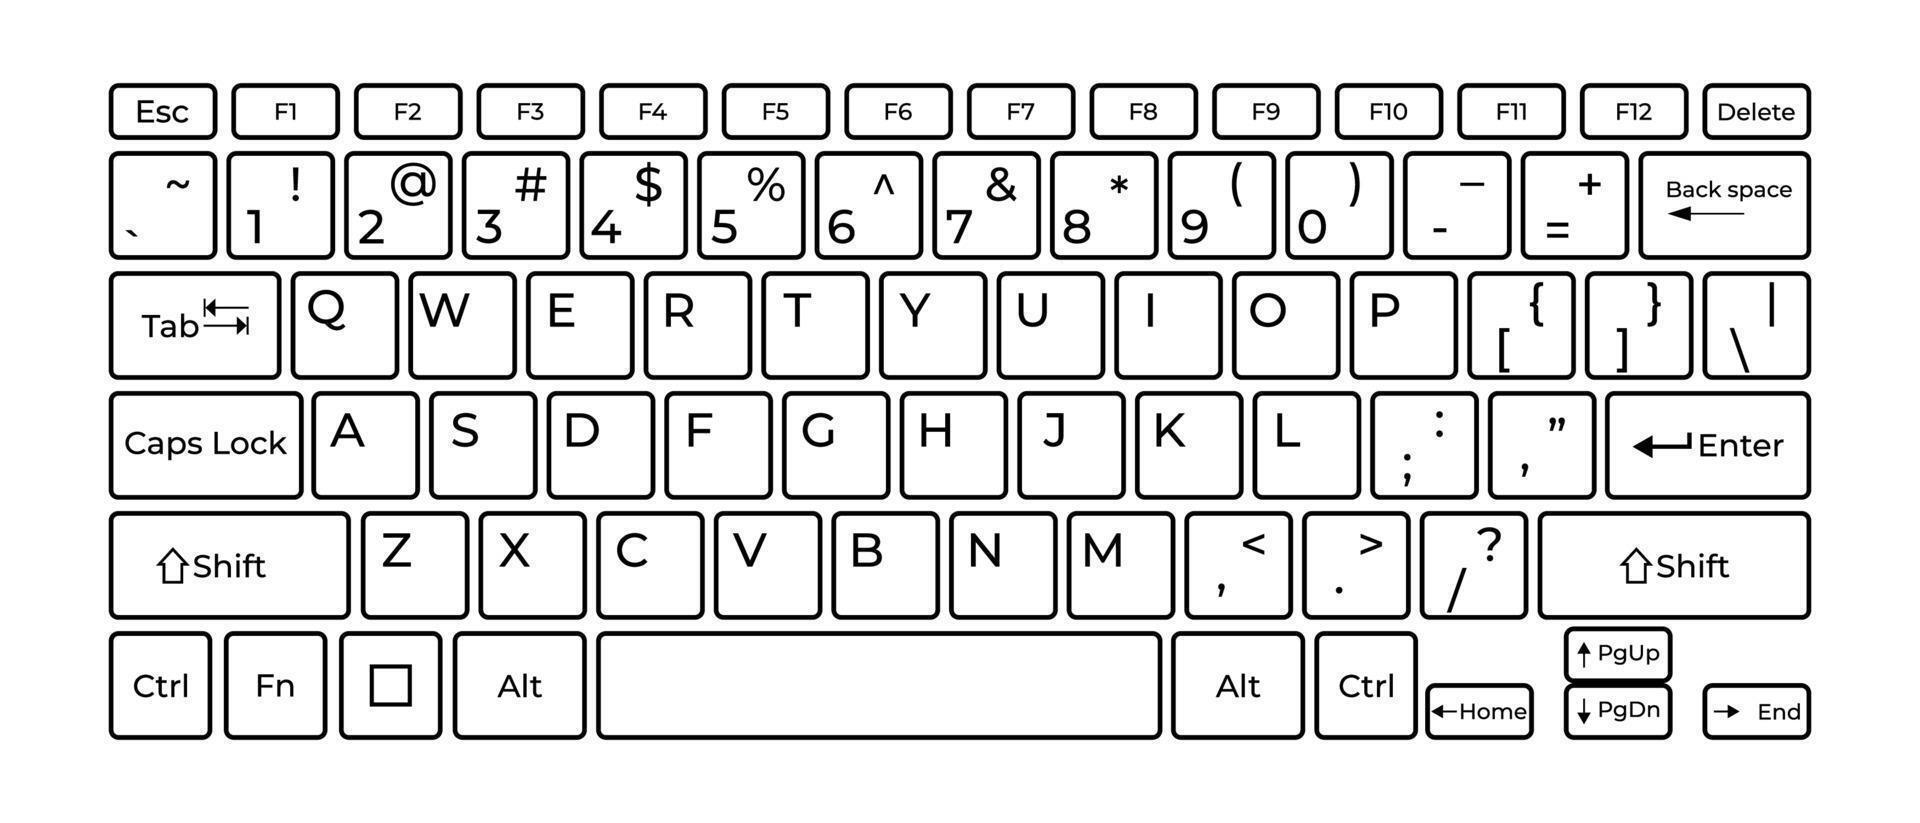
\includegraphics[width=0.7\textwidth]{Images/teclado.jpg}
    \caption{Imagen de un teclado}
    \label{fig:teclado}
\end{figure}
\subsection{Plataforma de despliegue}
Para el despliegue de este programa usaremos un ordenador, en el cual tengamos el contendor de \textit{Docker} instalado y encendido, y tambien por ultimo, que tenga la \textit{JDK 21}, instalada, además de que este
despliegue ocurrirá en un sistema Windows primero, y después se barajará la posibilidad de desplegarlo en sistemas \textit{Linux}, basados en \textit{Debian}.
\clearpage
\subsection{Arquitectura logica}
Estructura del proyecto en el diagrama de clases:
\subsubsection{Diagrama de clases}
% metemos la imagen de la carpeta images que se llama diagrama.png
\begin{figure}[ht]
    \centering
    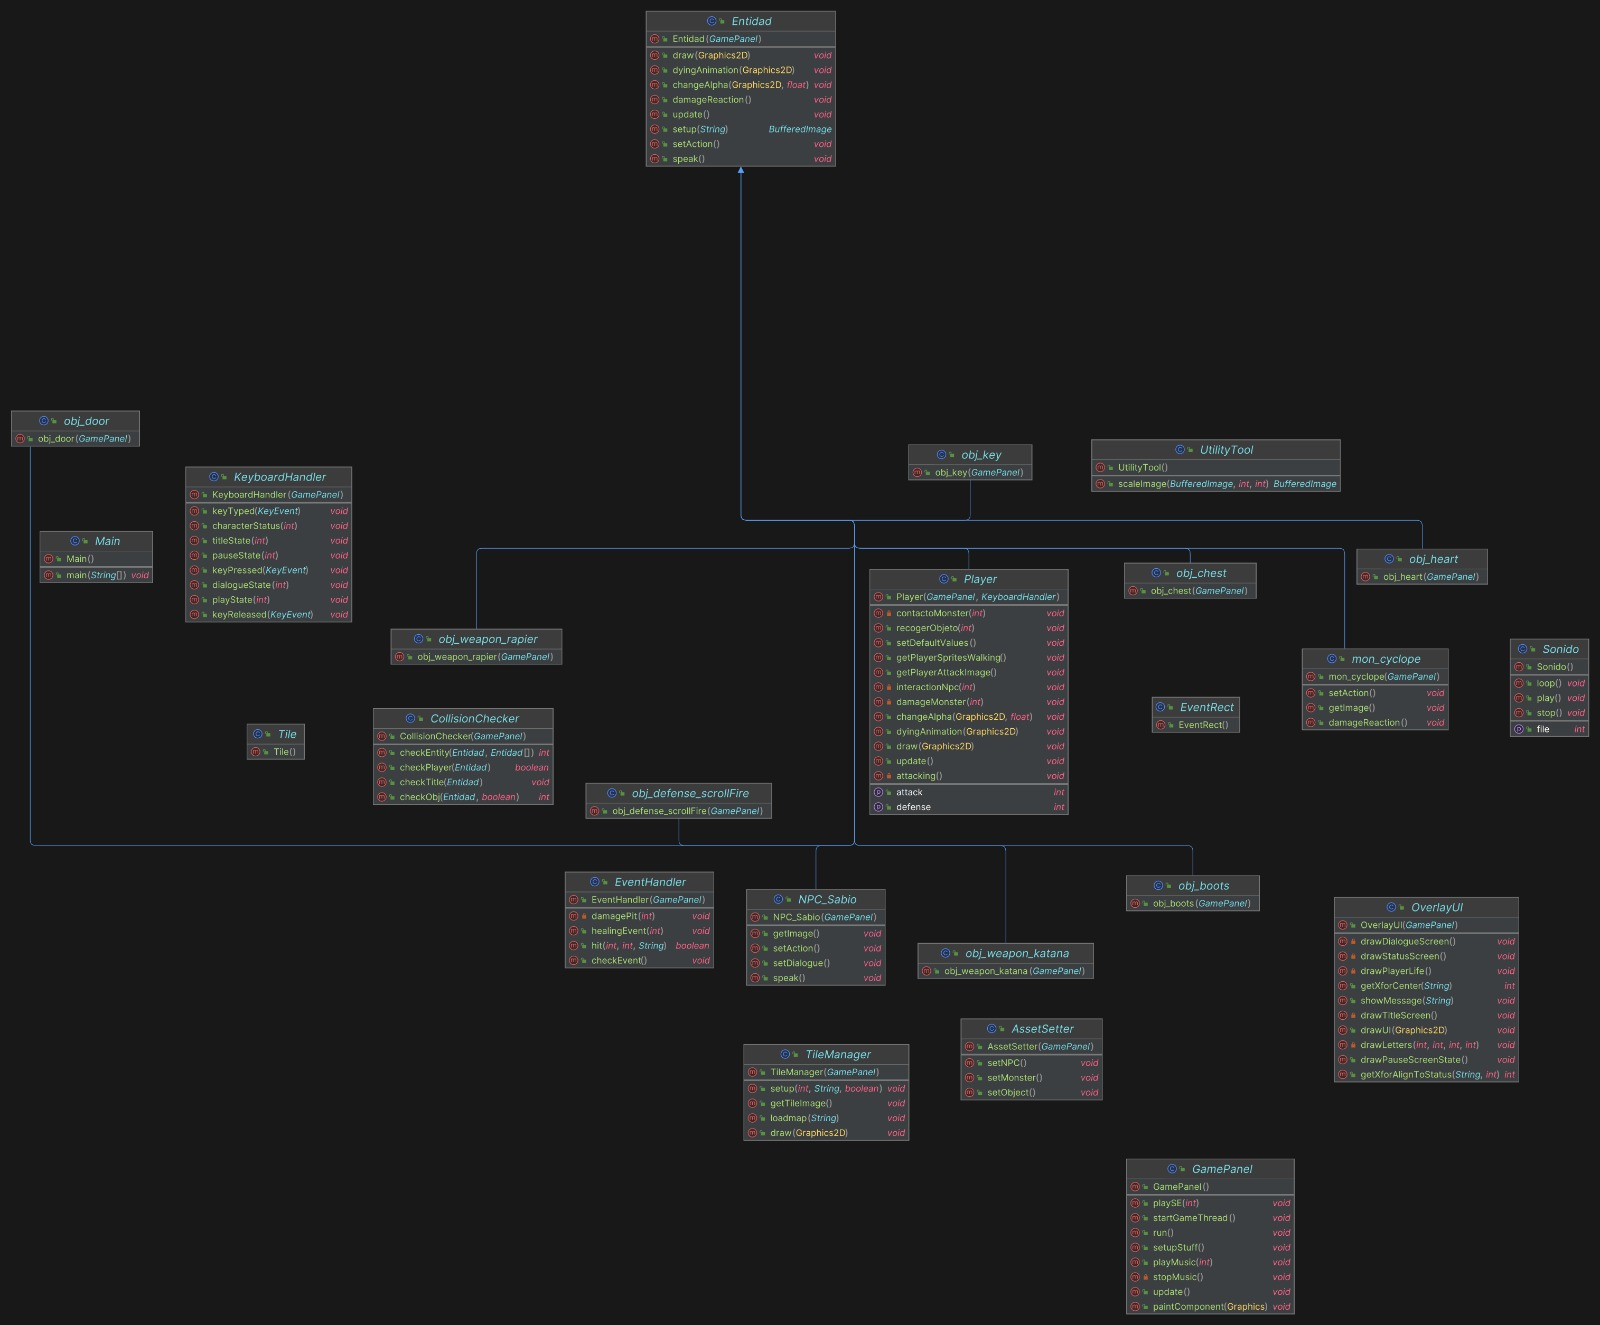
\includegraphics[width=0.7\textwidth]{Images/diagrama.jpg}
    \caption{Diagrama de clases}
    \label{fig:diagrama-clases}
\end{figure}

\subsubsection{Explicaciones del diagrama}
Como podemos ver en el diagrama, hay varias clases importantes a lo largo de la estructura del mismo, que son, \textbf{Player, Gamepanel y Entidad}, estas clases son las más importantes ya que
nos ayudan a definir muchas cosas.\\
En el caso de \textit{Entidad}, nos permite desarrollar enemigos, objetos, npc y el propio jugador, ya que estos objetos, extienden de \textit{Entidad}, lo que deja que esta clase sea una clase llena de atributos.
\subsubsection{Metodo run}
En cuanto a \textit{Gamepanel}, esta clase sería la encargada de tener el panel de juego y conectarse con todas las clases del proyecto, ya que, por ejemplo define
el tamaño de los assetts, el tamaño del texto, y varios aspectos más de dentro del juego, esta clase además es de las más importantes ya que contiene parte de los metodos más criticos del proyecto como por ejemplo el siguiente.\\
\begin{figure}[ht]
    \centering
    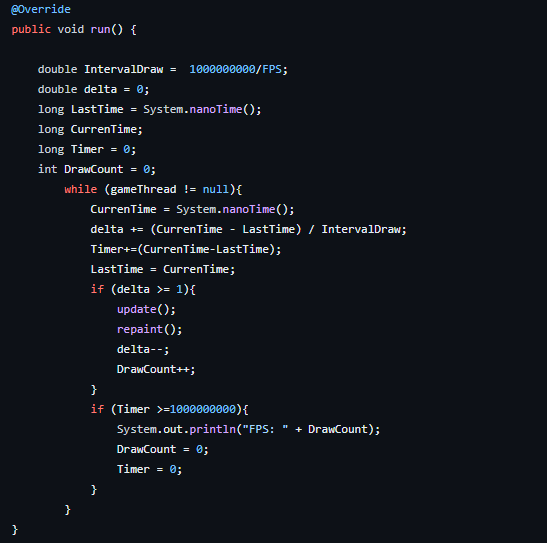
\includegraphics[width=0.7\textwidth]{Images/fpsMethod.PNG}
    \caption{Método del hilo principal}
    \label{fig:metodos}
\end{figure}
\\
Este método empieza inicializando 6 variables que le servirán para calcular un \textit{delta}, para ello hace uso de esta ecuación:
$$\text{IntervalDraw} = \frac{1}{\text{FPS}}$$
Como vemos esta ecuación sería la inversa de los \textit{FPS o Frames per Second}, dicho esto explicaremos cada variable.
\begin{itemize}
    \item \textit{IntervalDraw:} esta variable es la encargada de calcular en nanosegundos el tiempo necesario para dibujar un fotograma a la velocidad deseada
    \item \textit{delta:} Lleva un seguimiento del tiempo transcurrido desde el último fotograma.
    \item \textit{LastTime:} Almacena el tiempo en nanosegundos en el que se procesó el último fotograma.
    \item \textit{CurrenTime:} Almacena el tiempo actual en nanosegundos.
    \item \textit{Timer:} Lleva el seguimiento del tiempo transcurrido.
    \item \textit{DrawCount:} Es el contador de FPS del juego.
\end{itemize}
\textbf{Bucle principal}\\
Esta parte del codigo, ejecuta un bucle (El bucle se ejecuta mientras gameThread no sea nulo (es decir, mientras el juego esté funcionando)) en el cual ocurre lo siguiente:
\begin{itemize}
    \item Se actualiza el valor de CurrenTime.
    \item Se calcula el tiempo transcurrido desde el último fotograma y se agrega a delta.
    \item Se actualiza el valor de LastTime.
    \item Si delta supera 1, se llama a los métodos update() y repaint() para actualizar y dibujar el siguiente fotograma.
    \item Se decrementa delta en 1 y se incrementa DrawCount.
    \item Si Timer supera 1 segundo (1,000,000,000 nanosegundos), se muestra el número de fotogramas dibujados en la consola y se reinician los contadores.
\end{itemize}
Es decir, este metodo controla la lógica del dibujado o render del juego para que sea siempre de 60 fotogramas por segundo, es decir, dibuja 60 veces por segundo lo que tenemos en pantalla
de esta manera no tenemos valores extremadamente altos que no sirve de nada tener en un juego de este estilo.\\
Acabando con las clases principales, tenemos la clase \textit{Player} la cual tiene todos los metodos relacionados al jugador, es decir, el metodo de atacar, el metodo de moverse, colisiones con objetos,
etc \dots
\clearpage
\subsubsection{Método loadmap}
Aun asi, vale la pena destacar varios metodos interesantes como el de \textit{"loadmap"}, que encontramos en la clase \textit{"TileMananger"}, la clase encargada de leer el mapa del juego.
\begin{figure}[ht]
    \centering
    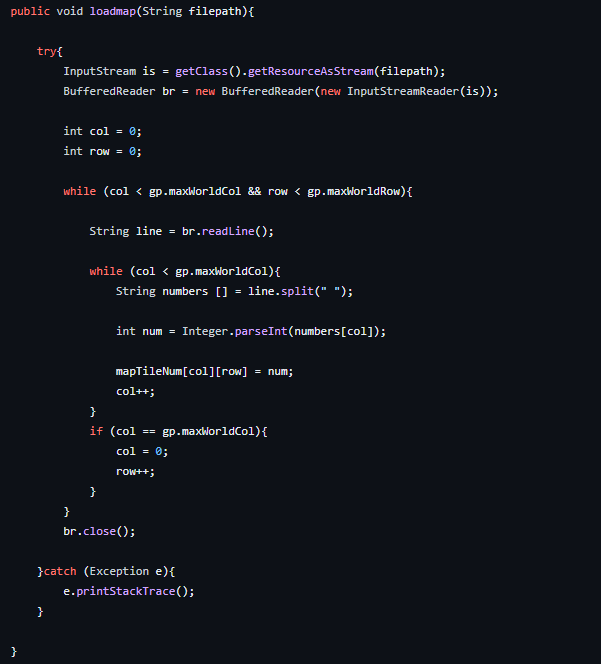
\includegraphics[width=0.7\textwidth]{Images/loadmap.PNG}
    \caption{Método de carga de mapas}
    \label{fig:metodos}
\end{figure}
\\
\textbf{Explicacion del metodo}\\
Este metodo funciona de la siguiente manera, a modo de resumen, lee el archivo .txt del mapa que esta compuesto solo de numeros y a cada numero le asigna una casilla, de esta manera, según el numero la casilla
tiene una imagen u otra.\\
Ahora de forma extensa, explicaremos paso por paso que hace este metodo:
\begin{enumerate}
    \item El método toma una cadena, \textit{"filepath"}, esta cadena se refiere a la ubicación del mapa en el sistema de archivos del ordenador, es decir, la ruta del archivo
    \item "InputStream is = getClass().getResourceAsStream(filepath); BufferedReader br = new BufferedReader(new InputStreamReader(is));" esta parte del codigo lo que hace es crear un BufferReader que lee el archivo del mapa.
    \item "getClass().getResourceAsStream(filepath)" lo que hace es localizar el archivo en el sistema.
    \item Las variables \textit{row} y \textit{col} nos sirven para saber en que posición del mapa se encuentra.
    \item "while (col < gp.maxWorldCol \&\& row < gp.maxWorldRow)" el bucle continua mientras no se llegue al final del mapa
    \item "String line = br.readLine();" simplemente lee una linea del archivo
    \item "while (col < gp.maxWorldCol)" el bucle se ejecuta para cada columna actual
    \item "String numbers [] = line.split(" "); int num = Integer.parseInt(numbers[col]); mapTileNum[col][row] = num; col++;" aquí se divide la línea en números, se convierte cada número a un entero y se almacena en el array \textit{mapTileNum}
    \item "if (col == gp.maxWorldCol){ col = 0; row++; }" Cuando se ha llegado al final de una fila, se incrementa la variable \textit{row} y se reinicia la variable \textit{col}
    \item "br.close();" cierra el BufferReader
    \item Y por ultimo el catch captura la excepcion en caso de que se produzca
\end{enumerate}
Este es un metodo muy curioso ya que puede producir otra excepción más que no he controlado, estamos hablando de la famosa excepción \textit{java.lang.OutOfMemoryError}, debido a que si tenemos un mapa muy grande
la máquina virtual de java, \textit{JVM} se queda sin memoria en el heap y detiene el programa porque ha "roto".
\clearpage
\subsubsection{Método draw}
Otro método interesante sería el método \textit{"draw"} de nuevo de la clase \textit{"TileMananger"}, el cual se encarga de dibujar las "casillas" de juego.\\
De forma resumida, va dibujando las casillas en la posición determinada en el mapa del juego.\\
\textbf{Explicación del método}\\
Este método es bastante simple de entender si hemos entendido los anteriores, por lo que procederemos a su desglose:
\begin{enumerate}
    \item "public void draw(Graphics2D g2)" primero recibe un objeto del tipo Graphics2D como argumento que usará para dibujar en pantalla.
    \item "worlCol y worlRow" son las variables que usaremos para rastrear la posición en la que nos encontramos
    \item "while(Wordlcol < gp.maxWorldCol \&\& WorldRow < gp.maxWorldRow)" este bucle continua mientras no lleguemos al final del mapa
    \item "int tileNum = mapTileNum[Wordlcol][WorldRow]" y aqui obtenemos el número de la casilla que se va a dibujar
    \item \texttt{int worldX = Wordlcol * gp.tileSize; int worldy = WorldRow * gp.tileSize} aquí calculamos las coordenadas \texttt{x} e \texttt{y} del juego
    \item "int screenX = worldX - gp.player.wordlx + gp.player.ScreenX; int screenY = worldy - gp.player.wordly + gp.player.ScreenY" aqui se calculan las coordenadas de la pantalla
    \item "g2.drawImage(tile[tileNum].image,screenX,screenY, null);" aqui dibujamos la casilla
    \item Incrementamos las columnas de la variable que rastrea las columnas
    \item "if (Wordlcol == gp.maxWorldCol){ Wordlcol = 0; WorldRow++; }" cuando se ha llegado al final de una fila, se incrementa la variable WorldRow y se reinicia la variable Wordlcol
\end{enumerate}
\begin{figure}[ht]
    \centering
    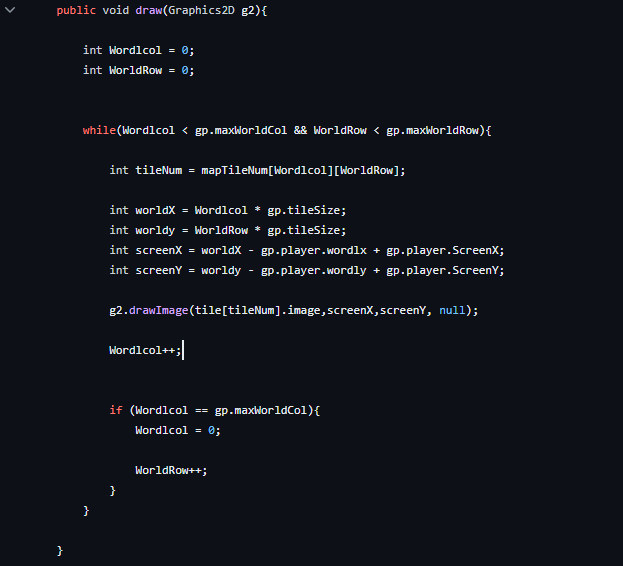
\includegraphics[width=0.6\textwidth]{Images/draw.PNG}
    \caption{Método de dibujado de mapas}
    \label{fig:metodos}
\end{figure}


\clearpage
% ------------------------------------------------
\subsection{Diagrama de casos de uso}
En el diagrama de casos de uso, tenemos un actor que seria el jugador. Este actor realizaría varias funciones:
\begin{itemize}
    \item Crear una partida
    \item Cargar una partida
    \item Empezar el juego
    \item Mover el personaje
    \item Pausar el juego
    \item Ver el estado del personaje
    \item Salir del juego
    \item Activar eventos
    \item Combatir
    \item Interactuar con NPCs
    \item Obtener objetos, experiencia, dinero.
    \item Comprar y Vender objetos
    \item Interactuar con el entorno
\end{itemize}

Insertar imagen del diagrama UML

\clearpage



\section{Desarrollo realizado}
Para el desarrollo del proyecto hemos usado las siguientes herramientas:
\begin{itemize}
    \item IntelliJ
    \item Docker
    \item Jooq
    \item JDK 21
    \item Visual studio Code
    \item \LaTeX
    \item Excalidraw
    \item Github Repositories
    \item MySQL
\end{itemize}
Ahora pasaremos a los detalles del codigo.
\subsection{Detalles del codigo desarrollado}
Empezaremos describiendo lo que realiza la clase principal, la clase \textit{"Main"}, cuyo codigo es:
\begin{lstlisting}
    package main;

import javax.swing.*;
import java.awt.*;

public class Main {
    public static void main(String args[]){
        JFrame win = new JFrame();
        win.setDefaultCloseOperation(JFrame.EXIT_ON_CLOSE);
        win.setResizable(false);
        //win.setBackground(Color.black);
        win.setTitle("Eldoria");

        GamePanel gpanel = new GamePanel();
        win.add(gpanel);

        win.pack();

        win.setLocationRelativeTo(null);
        win.setVisible(true);
        gpanel.setupStuff();
        gpanel.startGameThread();

    }
}
\end{lstlisting}
Dentro de este codigo encontramos varios aspectos a destacar, el primero es que estamos creando un JFrame en primera instancia y luego le estamos diciendo tambien que al darle a la "X", nos cierre el programa automaticamente.
Continuamos diciendole que no queremos un resize de la ventana actual del juego, por eso el false, seguimos con el titulo, y a continuacion la instancia de GamePanel, la cual nos servirá para instanciar más cosas.
Centramos la ventana con el setLocationRelativeTo, la hacemos visible y le decimos a GamePanel que vaya dibujando ciertas cosas del videojuego e inicie el hilo principal del juego.

\clearpage
% -----------------------------------
\section{Bibliografia}
% Haz un listado de las fuentes que has usado para realizar el proyecto
\begin{itemize}
    \item \textbf{Repositorio del juego} - \url{https://github.com/Pisa-17/TFG-DAM-Eldoria/tree/main}
    \item \textbf{Excalidraw} - \url{https://excalidraw.com/}
    \item \textbf{Manual LaTeX} - \url{https://manualdelatex.com/}
    \item \textbf{Mermaid} - \url{https://mermaid.js.org/intro/getting-started.html}
    \item \textbf{IntelliJ} - \url{https://www.jetbrains.com/es-es/idea/}
    \item \textbf{Editor Pixelart} - \url{https://www.piskelapp.com/}
    \item \textbf{Como hacer Assets} - \url{https://tips.clip-studio.com/es-es/articles/2484}
    \item \textbf{TFG de la Escuela de Segovia} - \url{https://uvadoc.uva.es/bitstream/handle/10324/24495/TFG-B%201042.pdf?sequence=1}
    \item \textbf{Docker} - \url{https://www.docker.com/}
    \item \textbf{Imagen Docker MySQL} - \url{https://hub.docker.com/_/mysql/}
    \item \textbf{Out Of Memory Error} - \url{https://stackoverflow.com/questions/1596009/java-lang-outofmemoryerror-java-heap-space}
    \item \textbf{Assets} - \url{https://pixel-boy.itch.io/ninja-adventure-asset-pack}
    \item \textbf{Autor de los Assets} - \url{https://twitter.com/2Pblog1}
    \item \textbf{JooQ} - \url{https://www.jooq.org/}
    \item \textbf{Visual Studio Code} - \url{https://code.visualstudio.com/Download}
    \item \textbf{Diagrama de clases IntelliJ} - \url{https://www.jetbrains.com/help/idea/class-diagram.html}
    \item \textbf{JDK 21} - \url{https://www.oracle.com/java/technologies/javase/jdk21-archive-downloads.html}
    \item \textbf{Retro Art Article} - \url{https://medium.com/@dq_irfandi/the-nostalgia-effect-how-retro-games-influence-modern-gaming-8925be77694e}
    \item \textbf{Why retro games are so Loved?} - \url{https://www.wired.com/story/why-retro-looking-games-get-so-much-love/}
    \item \textbf{How to list code in LaTeX} - \url{https://es.overleaf.com/learn/latex/Code_listing}
    \item \textbf{Libro - The Legend of Zelda Hyrule historia} - \url{https://en.wikipedia.org/wiki/The_Legend_of_Zelda:_Hyrule_Historia} - ISBN 978-1-61655-041-7
\end{itemize}

\clearpage
% ----------------------------------------

\begin{appendices}
    \renewcommand{\thesection}{} % Elimina la numeración de las secciones

    \section{Anexo I - Manual de Usuario}
    Los controles del juego son bastante simples, tendriamos las teclas \textit{W,A,S y D}, para mover el personaje y las teclas \textit{C, P, y ENTER} para otras acciones.
    \begin{itemize}
        \item W - Mover el personaje hacia arriba
        \item A - Mover el personaje a la izquierda
        \item D - Mover el personaje a la derecha
        \item S - Mover el personaje hacia abajo
        \item C - Ver las estadisticas del personaje
        \item P - Abrir el menu de Pausa
        \item ENTER - Interactuar con NPCs, atacar, aceptar o continuar.
    \end{itemize}
    \clearpage
    % ---------------------------------------

    \section{Anexo II - Assets}
    Aquí va el contenido del segundo anexo...
    \clearpage
    % ---------------------------------------

    \section{Anexo III - Arte e inspiraciones detalladas}
    Dentro del apartado artistico debemos remontarnos a una época pasada, ya que tomamos muchos aspectos de juegos de décadas anteriores que nos han ayudado en cuanto a diseño, estética y cómo se ha
    diseñado el juego.

    \subsection{The legend of Zelda}
    Empezamos por la primera y clara inspiración que es \textit{The legend Of Zelda}, este videojuego bastante importante en la industria, sentó las bases para los próximos videojuegos de los siguientes años
    y es día de hoy que su fórmula sigue siendo un exito. La fórmula de este juego nos presenta una aventura de un héroe que debe rescatar a una princesa de un rey malvado, para ello durante la aventura se ganará
    el favor de las diosas de su mundo así como una espada sagrada para poder derrotar a este rey malvado. Esta fórmula gana mucho cuando nos metemos de lleno al juego, y dentro del juego lo que encontramos son puzzles,
    puzzles que nos proponen desafíos para superar las mazmorras y conseguir objetos. En los años 80 fue uno de los juegos más importantes.

    \subsection{Final fantasy}
    La segunda inspiración tomada es otro juego de los años 80, el cual se llama \textit{Final Fantasy}, este juego se trata de un juego en dos dimensiones RPG por turnos que nos presenta una historia,
    acerca de 4 muchachos que se embarcan en la búsqueda de unos cristales mágicos que les servirán para disipar el mal de su mundo, durante la aventura se enfrentan a enemigos formidables y el juego tiene
    una estética de fantasía medieval. A dia de hoy esta saga sigue en desarollo, actualmente han sacado 16 juegos principales y varios secundarios.

    \subsection{Blasphemous}
    La tercera inspiración ha sido un juego que se sale de los generos de RPG, se trata de un juego metroidvania, desarrollado en España, se trata de \textit{Blasphemous},
    un juego en dos dimensiones que nos pone en la piel del penitente, el cual entrará en un camino de penitencia y tendrá que realizar humillaciones para devolver el orden a su mundo, Cvstodia.
    Este juego presenta inspiración en mi proyecto ya que se trata de un juego con estética \textit{pixel art}, que es relativamente reciente.

    \subsection{Arte del juego}
    El arte del juego sería una mezcla de todos los juegos ya mencionados excepto Blasphemous, ya que este último cuenta con sprites muy bien detallados y de mayor resolución.
    Se supone que el juego se desarrolla en una época medieval en la que existen magias, caballeros, dragones, ciclopes, etc \dots

    \clearpage
    % ---------------------------------------

    \section{Anexo IV - Vocablos usados}
    Durante este documento se han hecho uso de varios vocablos de los que seguramente se desconozca el significado, tales como "FPS" por ejemplo, por ello vamos a recopilarlos aqui junto a su definicion.
    \begin{itemize}
        \item FPS Frames per second - Imagenes que dibuja el programa por segundo, un frame es toda la imagen que dibuja el programa entera, con el personaje, el mapa, los objetos, etc \dots
        \item RPG Role playing game - Acrónimo asociado a los juegos de Rol
        \item NPC Non Playable Character - Personaje no jugable, suelen ser personajes con los que podemos hablar o Interactuar
        \item Inputs - Se refiere a las entradas del usuario al programa
        \item Pixel art - Estética basada en dibujar con pixeles solamente sin ningun arco o elemento circular
        \item Retro - Se refiere a una estética antigua, por ejemplo la de los juegos de los años 80
        \item Sprites - Son un conjunto de imágenes que representan un objeto o personaje
    \end{itemize}
    \clearpage
    % ---------------------------------------

\end{appendices}

\end{document}